\documentclass{standalone}
\usepackage{tikz}
\usetikzlibrary{patterns, positioning}


\begin{document}
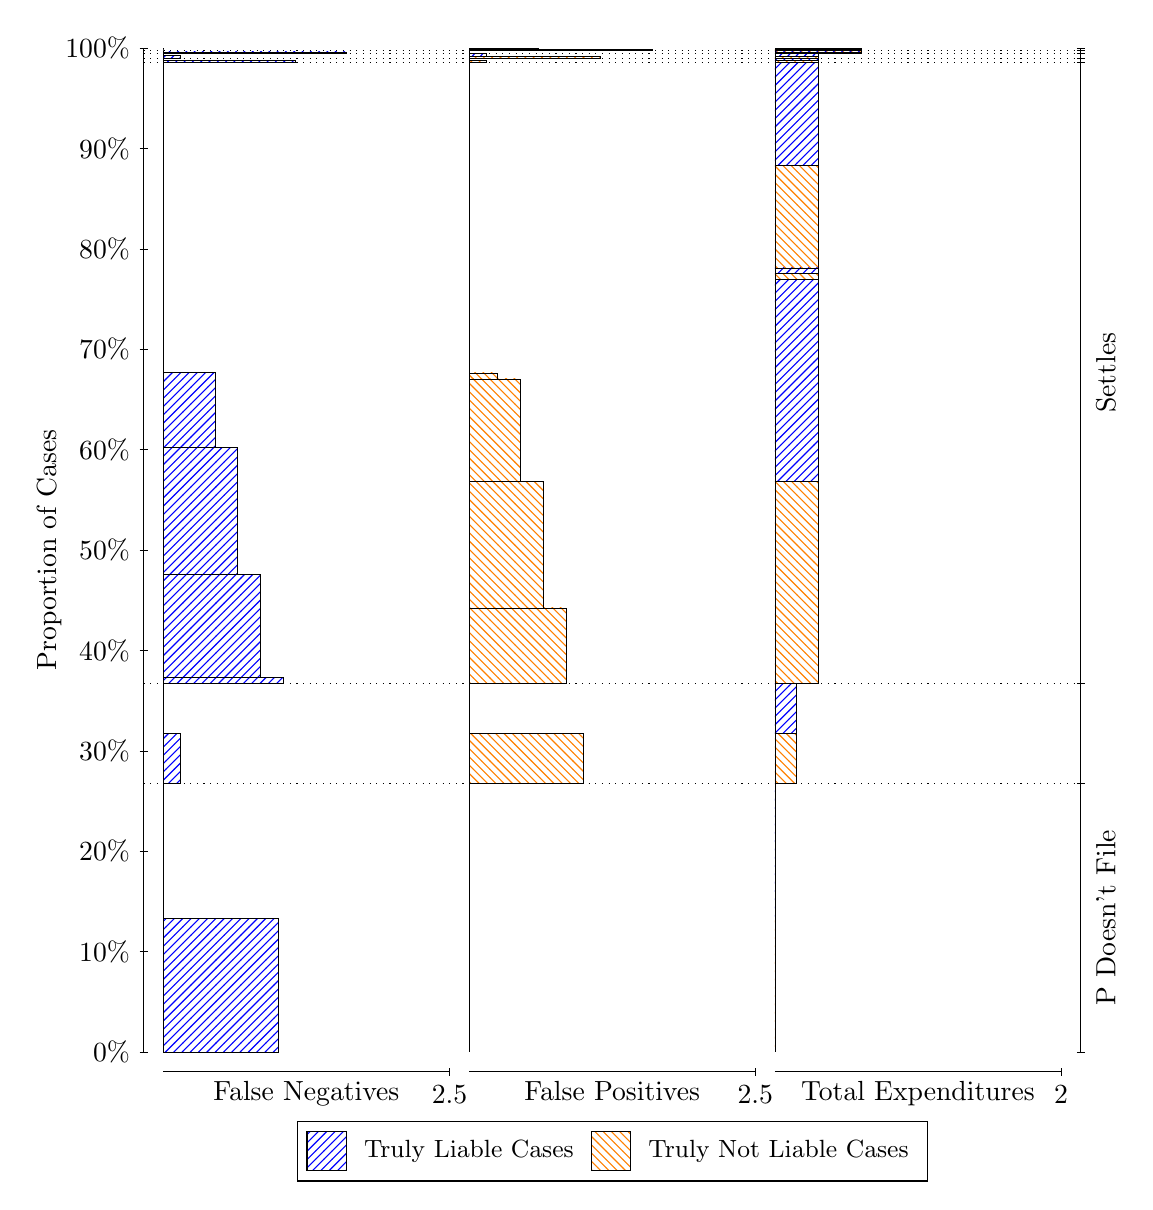
\begin{tikzpicture}
\draw[black, very thin] (1.5,1.75) -- (1.5,14.5);
\node[rotate=90, text=black, anchor=center] at (0.3, 8.125) {Proportion of Cases};
\draw[black, very thin] (1.45,1.75) -- (1.55,1.75);
\node[text=black, anchor=east] at (1.45, 1.75) {0\%};
\draw[black, very thin] (1.45,3.025) -- (1.55,3.025);
\node[text=black, anchor=east] at (1.45, 3.025) {10\%};
\draw[black, very thin] (1.45,4.3) -- (1.55,4.3);
\node[text=black, anchor=east] at (1.45, 4.3) {20\%};
\draw[black, very thin] (1.45,5.575) -- (1.55,5.575);
\node[text=black, anchor=east] at (1.45, 5.575) {30\%};
\draw[black, very thin] (1.45,6.85) -- (1.55,6.85);
\node[text=black, anchor=east] at (1.45, 6.85) {40\%};
\draw[black, very thin] (1.45,8.125) -- (1.55,8.125);
\node[text=black, anchor=east] at (1.45, 8.125) {50\%};
\draw[black, very thin] (1.45,9.4) -- (1.55,9.4);
\node[text=black, anchor=east] at (1.45, 9.4) {60\%};
\draw[black, very thin] (1.45,10.675) -- (1.55,10.675);
\node[text=black, anchor=east] at (1.45, 10.675) {70\%};
\draw[black, very thin] (1.45,11.95) -- (1.55,11.95);
\node[text=black, anchor=east] at (1.45, 11.95) {80\%};
\draw[black, very thin] (1.45,13.225) -- (1.55,13.225);
\node[text=black, anchor=east] at (1.45, 13.225) {90\%};
\draw[black, very thin] (1.45,14.5) -- (1.55,14.5);
\node[text=black, anchor=east] at (1.45, 14.5) {100\%};

\draw[black, very thin] (13.4,1.75) -- (13.4,14.5);
\draw[black, very thin] (13.35,1.75) -- (13.45,1.75);
\node[anchor=west] at (13.35, 1.75) {};
\draw[black, very thin] (13.35,5.1596) -- (13.45,5.1596);
\node[anchor=west] at (13.35, 5.1596) {};
\draw[black, very thin] (13.35,6.4346) -- (13.45,6.4346);
\node[anchor=west] at (13.35, 6.4346) {};
\draw[black, very thin] (13.35,14.32) -- (13.45,14.32);
\node[anchor=west] at (13.35, 14.32) {};
\draw[black, very thin] (13.35,14.372) -- (13.45,14.372);
\node[anchor=west] at (13.35, 14.372) {};
\draw[black, very thin] (13.35,14.436) -- (13.45,14.436);
\node[anchor=west] at (13.35, 14.436) {};
\draw[black, very thin] (13.35,14.468) -- (13.45,14.468);
\node[anchor=west] at (13.35, 14.468) {};
\draw[black, very thin] (13.35,14.5) -- (13.45,14.5);
\node[anchor=west] at (13.35, 14.5) {};

\draw[black, very thin, pattern color=blue, pattern=north east lines] (1.75,1.75) rectangle (3.2033,3.4434);
\draw[black, very thin, pattern color=orange, pattern=north west lines] (1.75,3.4434) rectangle (1.75,5.1596);
\draw[black, very thin, pattern color=blue, pattern=north east lines] (1.75,5.1596) rectangle (1.968,5.7971);
\draw[black, very thin, pattern color=orange, pattern=north west lines] (1.75,5.7971) rectangle (1.75,6.4346);
\draw[black, very thin, pattern color=blue, pattern=north east lines] (1.75,6.4346) rectangle (3.276,6.5059);
\draw[black, very thin, pattern color=blue, pattern=north east lines] (1.75,6.5059) rectangle (2.9853,7.8152);
\draw[black, very thin, pattern color=blue, pattern=north east lines] (1.75,7.8152) rectangle (2.6947,9.4237);
\draw[black, very thin, pattern color=blue, pattern=north east lines] (1.75,9.4237) rectangle (2.404,10.38);
\draw[black, very thin, pattern color=orange, pattern=north west lines] (1.75,10.38) rectangle (1.75,14.32);
\draw[black, very thin, pattern color=blue, pattern=north east lines] (1.75,14.32) rectangle (3.4213,14.346);
\draw[black, very thin, pattern color=orange, pattern=north west lines] (1.75,14.346) rectangle (1.75,14.372);
\draw[black, very thin, pattern color=blue, pattern=north east lines] (1.75,14.372) rectangle (1.968,14.411);
\draw[black, very thin, pattern color=orange, pattern=north west lines] (1.75,14.411) rectangle (1.75,14.436);
\draw[black, very thin, pattern color=blue, pattern=north east lines] (1.75,14.436) rectangle (4.0753,14.452);
\draw[black, very thin, pattern color=orange, pattern=north west lines] (1.75,14.452) rectangle (1.75,14.468);
\draw[black, very thin, pattern color=orange, pattern=north west lines] (1.75,14.468) rectangle (1.75,14.482);
\draw[black, very thin, pattern color=blue, pattern=north east lines] (1.75,14.482) rectangle (1.75,14.5);
\draw[black, very thin, pattern color=orange, pattern=north west lines] (5.6333,1.75) rectangle (5.6333,3.4663);
\draw[black, very thin, pattern color=blue, pattern=north east lines] (5.6333,3.4663) rectangle (5.6333,5.1596);
\draw[black, very thin, pattern color=orange, pattern=north west lines] (5.6333,5.1596) rectangle (7.0867,5.7971);
\draw[black, very thin, pattern color=blue, pattern=north east lines] (5.6333,5.7971) rectangle (5.6333,6.4346);
\draw[black, very thin, pattern color=orange, pattern=north west lines] (5.6333,6.4346) rectangle (6.8687,7.3909);
\draw[black, very thin, pattern color=orange, pattern=north west lines] (5.6333,7.3909) rectangle (6.578,8.995);
\draw[black, very thin, pattern color=orange, pattern=north west lines] (5.6333,8.995) rectangle (6.2873,10.297);
\draw[black, very thin, pattern color=orange, pattern=north west lines] (5.6333,10.297) rectangle (5.9967,10.374);
\draw[black, very thin, pattern color=blue, pattern=north east lines] (5.6333,10.374) rectangle (5.6333,14.32);
\draw[black, very thin, pattern color=orange, pattern=north west lines] (5.6333,14.32) rectangle (5.8513,14.346);
\draw[black, very thin, pattern color=blue, pattern=north east lines] (5.6333,14.346) rectangle (5.6333,14.372);
\draw[black, very thin, pattern color=orange, pattern=north west lines] (5.6333,14.372) rectangle (7.3047,14.398);
\draw[black, very thin, pattern color=blue, pattern=north east lines] (5.6333,14.398) rectangle (5.8513,14.436);
\draw[black, very thin, pattern color=orange, pattern=north west lines] (5.6333,14.436) rectangle (5.6333,14.452);
\draw[black, very thin, pattern color=blue, pattern=north east lines] (5.6333,14.452) rectangle (5.6333,14.468);
\draw[black, very thin, pattern color=orange, pattern=north west lines] (5.6333,14.468) rectangle (7.9587,14.482);
\draw[black, very thin, pattern color=blue, pattern=north east lines] (5.6333,14.482) rectangle (6.5053,14.5);
\draw[black, very thin, pattern color=orange, pattern=north west lines] (9.5167,1.75) rectangle (9.5167,3.4663);
\draw[black, very thin, pattern color=blue, pattern=north east lines] (9.5167,3.4663) rectangle (9.5167,5.1596);
\draw[black, very thin, pattern color=orange, pattern=north west lines] (9.5167,5.1596) rectangle (9.7892,5.7971);
\draw[black, very thin, pattern color=blue, pattern=north east lines] (9.5167,5.7971) rectangle (9.7892,6.4346);
\draw[black, very thin, pattern color=orange, pattern=north west lines] (9.5167,6.4346) rectangle (10.062,8.995);
\draw[black, very thin, pattern color=blue, pattern=north east lines] (9.5167,8.995) rectangle (10.062,11.56);
\draw[black, very thin, pattern color=orange, pattern=north west lines] (9.5167,11.56) rectangle (10.062,11.637);
\draw[black, very thin, pattern color=blue, pattern=north east lines] (9.5167,11.637) rectangle (10.062,11.708);
\draw[black, very thin, pattern color=orange, pattern=north west lines] (9.5167,11.708) rectangle (10.062,13.01);
\draw[black, very thin, pattern color=blue, pattern=north east lines] (9.5167,13.01) rectangle (10.062,14.32);
\draw[black, very thin, pattern color=orange, pattern=north west lines] (9.5167,14.32) rectangle (10.062,14.346);
\draw[black, very thin, pattern color=blue, pattern=north east lines] (9.5167,14.346) rectangle (10.062,14.372);
\draw[black, very thin, pattern color=orange, pattern=north west lines] (9.5167,14.372) rectangle (10.062,14.398);
\draw[black, very thin, pattern color=blue, pattern=north east lines] (9.5167,14.398) rectangle (10.062,14.436);
\draw[black, very thin, pattern color=orange, pattern=north west lines] (9.5167,14.436) rectangle (10.607,14.452);
\draw[black, very thin, pattern color=blue, pattern=north east lines] (9.5167,14.452) rectangle (10.607,14.468);
\draw[black, very thin, pattern color=orange, pattern=north west lines] (9.5167,14.468) rectangle (10.607,14.482);
\draw[black, very thin, pattern color=blue, pattern=north east lines] (9.5167,14.482) rectangle (10.607,14.5);
\draw[black, dotted] (1.5,5.1596) -- (13.4,5.1596);
\draw[black, dotted] (1.5,6.4346) -- (13.4,6.4346);
\draw[black, dotted] (1.5,14.32) -- (13.4,14.32);
\draw[black, dotted] (1.5,14.372) -- (13.4,14.372);
\draw[black, dotted] (1.5,14.436) -- (13.4,14.436);
\draw[black, dotted] (1.5,14.468) -- (13.4,14.468);
\draw[black, very thin] (1.75,1.5) -- (5.3833,1.5);
\node[text=black, anchor=north] at (3.5667, 1.5) {False Negatives};
\draw[black, very thin] (5.3833,1.45) -- (5.3833,1.55);
\node[text=black, anchor=north] at (5.3833, 1.45) {2.5};

\draw[black, very thin] (5.6333,1.5) -- (9.2667,1.5);
\node[text=black, anchor=north] at (7.45, 1.5) {False Positives};
\draw[black, very thin] (9.2667,1.45) -- (9.2667,1.55);
\node[text=black, anchor=north] at (9.2667, 1.45) {2.5};

\draw[black, very thin] (9.5167,1.5) -- (13.15,1.5);
\node[text=black, anchor=north] at (11.333, 1.5) {Total Expenditures};
\draw[black, very thin] (13.15,1.45) -- (13.15,1.55);
\node[text=black, anchor=north] at (13.15, 1.45) {2};

\node[text=black, centered, rotate=90] at (13.72, 3.4548) {P Doesn't File};

\node[text=black, centered, rotate=90] at (13.72, 10.377) {Settles};





\draw (7.449999999999999,1.5) node[draw=none] (baseCoordinate) {};
\begin{scope}[align=center]
        \matrix[scale=0.5, draw=black, below=0.5cm of baseCoordinate, nodes={draw}, column sep=0.1cm]{
            \node[rectangle, draw, minimum width=0.5cm, minimum height=0.5cm, pattern color=blue, pattern=north east lines] {}; &
            \node[draw=none, font=\small, text=black] (B) {Truly Liable Cases}; &
            \node[rectangle, draw, minimum width=0.5cm, minimum height=0.5cm, pattern color=orange, pattern=north west lines] {}; &
            \node[draw=none, font=\small, text=black] (B) {Truly Not Liable Cases}; \\
            };
\end{scope}

\end{tikzpicture}
\end{document}